\section{Internet of Things}
\label{sec:iot}

Das Internet of Things (IoT) beschreibt im Generellen Geräte, die mit dem Internet verbunden sind; doch im engeren bezieht sich der Begriff vielmehr auf Geräte, welche zusätzlich dazu auch miteinander kommunizieren. Mit „Geräten“ sind in diesem Kontext sowohl simple Sensoren gemeint, als auch PCs, Smartphones oder tragbare Geräte wie Smartwatches.\\
Die Fähigkeiten und Möglichkeiten von IoT gehen allerdings über eine simple Verknüpfung hinaus. So ist es möglich, die Informationen, welche von dem Netzwerk an IoT Geräten gesammelt werden, zu analysieren und auszuwerten. Daraus können dann weiterführende Informationen gewonnen werden, oder diese Daten können Automatisierungssystemen als Eingabe gegeben werden.\\
Ein Beispiel für eine solche Verknüpfung und Automatisierung wäre ein Thermostat, welches die Temperatur anhand der Jahreszeit, der aktuellen Temperatur im Zimmer (gemessen über einen separaten Sensor) und der Präsenz einer Person (gemessen über die WLAN-Verbindung eines Smartphones) regelt. Die Stärke liegt hier also vorwiegend in der Verknüpfung verschiedener Datenquellen und Geräte.

Die Geräte in einem solchen Netzwerk kommunizieren oft über den Router des lokalen Netzes miteinander und gegebenenfalls übers Internet zu einem anderen Standort oder in die Cloud. Viele IoT Geräte benötigen dafür jedoch einen zusätzlichen Gateway.\\
Ein typisches IoT Heimnetzwerk ist in Grafik \ref{fig:IoT_Netzwerk} abgebildet. In diesem konkreten Beispiel wird neben der Cloud ein Heimserver im lokalen Netzwerk benutzt, um einige Anwendungen lokal auszuführen. So können unter anderem die Sicherheitskameraaufzeichnungen vollständig lokal gespeichert und verarbeitet werden, während die anderen Geräte ihre Daten an die Cloud weitergeben und auch von außerhalb des Netzwerkes gesteuert werden können.
%
\begin{figure}[htbp]
	\centering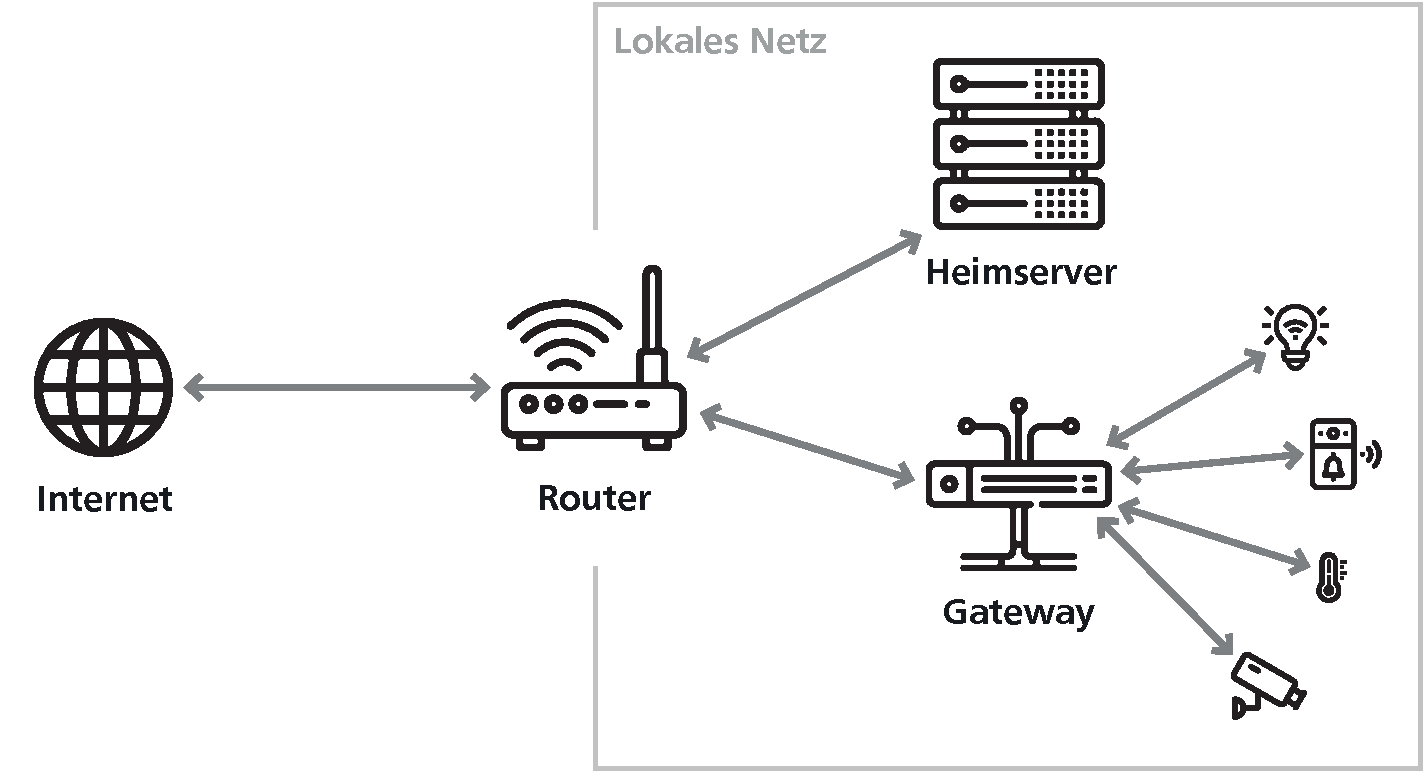
\includegraphics[width=0.9\textwidth]{images/02/IoT_Netzwerk.pdf}
    \caption{IoT Heimnetzwerk mit Heimserver}
    \label{fig:IoT_Netzwerk}
\end{figure}

Ermöglicht wurde diese durch IoT bedingte Trendwende neben der allgegenwärtigen Präsenz von Elektronik durch die weite Verbreitung von robusten, drahtlosen Netzwerken, sowie den immer weiter wachsenden Cloud-Infrastrukturen. Bei der Elektronik war eine wesentliche Neuerung die Verfügbarkeit von günstigen Allzweck-Prozessoren. Während zuvor noch oft spezialisiertere Hardware benutzt wurde, ist es mittlerweile vielmals günstiger, einen allgemeineren, massenproduzierten Chip zu verbauen [\cite{besprokeCpus}]. Ein weiterer Faktor ist IPv6 (Internet Protocol Version 6), wodurch es möglich wurde, nicht nur dem gesamten Netzwerk eines Hauses oder einer Wohnung eine IP-Adresse zuzuordnen, sondern jedem einzelnen Gerät.\\
Um es mit den Worten von Rakesh Kumar, Associate Professor für Elektro- und Computertechnik an der University of Illinois zu sagen: „Prozessoren sind für die meisten Anwendungen überdimensioniert“ [\cite{besprokeCpus}]. Im Falle von IoT ist dies aber von großem Vorteil, denn so ist es nicht nur für die Hersteller wesentlich einfacher und günstiger geworden, nicht funktionsnotwendige Technologien wie eine Programmschnittstelle (z.B. eine REST API, siehe Kapitel \ref{sec:rest}) in ihre Geräte einzubetten, sondern es ist auch für die Nutzer einfacher geworden solche Funktionalitäten im Nachhinein hinzuzufügen. So hat sich eine wachsende Gemeinschaft aufgebaut, welche sich damit beschäftigt, Geräte „smart“ zu machen und sie an eine Verbindung an ein IoT Netzwerk vorzubereiten.

\subsection{Verbreitung und Wachstum des Internet of Things}
\label{subsec:iot_verbreitung}

Um zu verdeutlichen, wie weitverbreitet, das Internet of Things und die dazugehörigen Geräte sind, zeigt Tabelle \ref{tab:iotRegierung} die Regierungsausgaben für IoT-Endgeräte und -Kommunikationsinfrastruktur, geordnet nach Anwendungsgebiet und in Milliarden US-Dollar. Die Tabelle beinhaltet dabei neben den historischen Daten für 2020 auch eine Vorhersage für die Jahre 2021 und 2022. Diese Daten beziehen sich zwar nur auf Regierungsausgaben, doch sie geben auch einen Hinweis auf die allgemeine Akzeptanz und Verbreitung von IoT Technologien.
%
\bgroup
\def\arraystretch{1.5}
\vspace{5mm}\begin{table}[htbp]
    \centering
    \begin{tabularx}{140mm}{@{}p{80mm}|*3{>{\centering\arraybackslash}X}@{}}
        \rowcolor{dikblue} \mbox{\color{white}\textbf{Anwendungsgebiet}} & \mbox{\color{white}\textbf{2020}} & \mbox{\color{white}\textbf{2021*}} & \mbox{\color{white}\textbf{2022*}} \\
        Außenüberwachung                & 9,3 & 9,7 & 12,0 \\ \hline
        Maut- und Verkehrsmanagement    & 1,8 & 2,1 & 2,6 \\ \hline
        Verfolgung von Stadt-Anlagen    & 1,5 & 1,9 & 2,2 \\ \hline
        Spurensicherung der Polizei     & 0,9 & 1,2 & 1,5 \\ \hline
        Parkraumverwaltung              & 0,5 & 0,6 & 0,7 \\ \hline
        Feuerwehrüberwachung            & 0,8 & 1,0 & 1,1 \\ \hline
        Andere                          & 0,8 & 1,0 & 1,2 \\ \hline
        \textbf{Gesamtmarkt} & \textbf{15,6} & \textbf{17,5} & \textbf{21,3} \\
    \end{tabularx}
    \caption{Regierungsausgaben für IoT-Endgeräte und -Kommunikationsinfrastruktur in Milliarden US-Dollar [\cite{iotGovernment}]}
    \label{tab:iotRegierung}
\end{table}
\egroup

Wie in Tabelle \ref{tab:iotRegierung} abzulesen ist, wird ein starkes Wachstum für die Regierungsausgaben für IoT prognostiziert. Um dieses Wachstum mehr in den Fokus zu rücken, werden im Diagramm \ref{fig:IoT_Ausgaben} die weltweiten Endbenutzerausgaben für IoT-Lösungen für die Jahre 2017 bis 2025 abgebildet. Die mit \verb|*| markierten Jahre symbolisieren hier Jahre, für die die Daten auf Grundlage des historischen Trends abgeschätzt wurden. Wie in dieser Grafik zu sehen ist, wird ein enormes und an Geschwindigkeit zunehmendes Wachstum im IoT Bereich prognostiziert.
%
\begin{figure}[htbp]
	\centering\includegraphics[width=1.0\textwidth]{images/02/IoT_Ausgaben.eps}
    \caption{Wachstum weltweiter Ausgaben für IoT-Lösungen [\cite{iotSpending}]}
    \label{fig:IoT_Ausgaben}
\end{figure}

\subsection{Industrial Internet of Things}
\label{subsec:iot_iiot}

Ein weiterer Einsatzpunkt für IoT-Anwendungen ist in Fabrik- und Industrieanlagen. Hier werden Geräte mit Sensoren ausgestattet, wodurch Metriken wie Auslastung, Materialverbrauch, Durchsatz, etc. genauer und automatisiert ausgelesen und analysiert werden können. Auch kann der Maschinenverschleiß besser im Auge behalten werden, was zu einer proaktiven, statt einer reaktiven Wartung und einer längeren Lebensdauer der Geräte führt. Diese Eigenschaften führen zu einer zunehmenden Automatisierung von Fabriken [\cite{iotAnderl}].

Da sich diese industriell orientierten Anwendungen in einigen Punkten von Anwendungen in anderen Gebieten unterscheidet, wird diese Unterkategorie des IoT auch als Industrial Internet of Things (IIoT) bezeichnet. In Grafik \ref{fig:IIoT_vs_IoT} sind einige dieser Unterschiede zwischen IIoT und Massenmarkt-IoT aufgezeigt.
%
\begin{figure}[htbp]
	\centering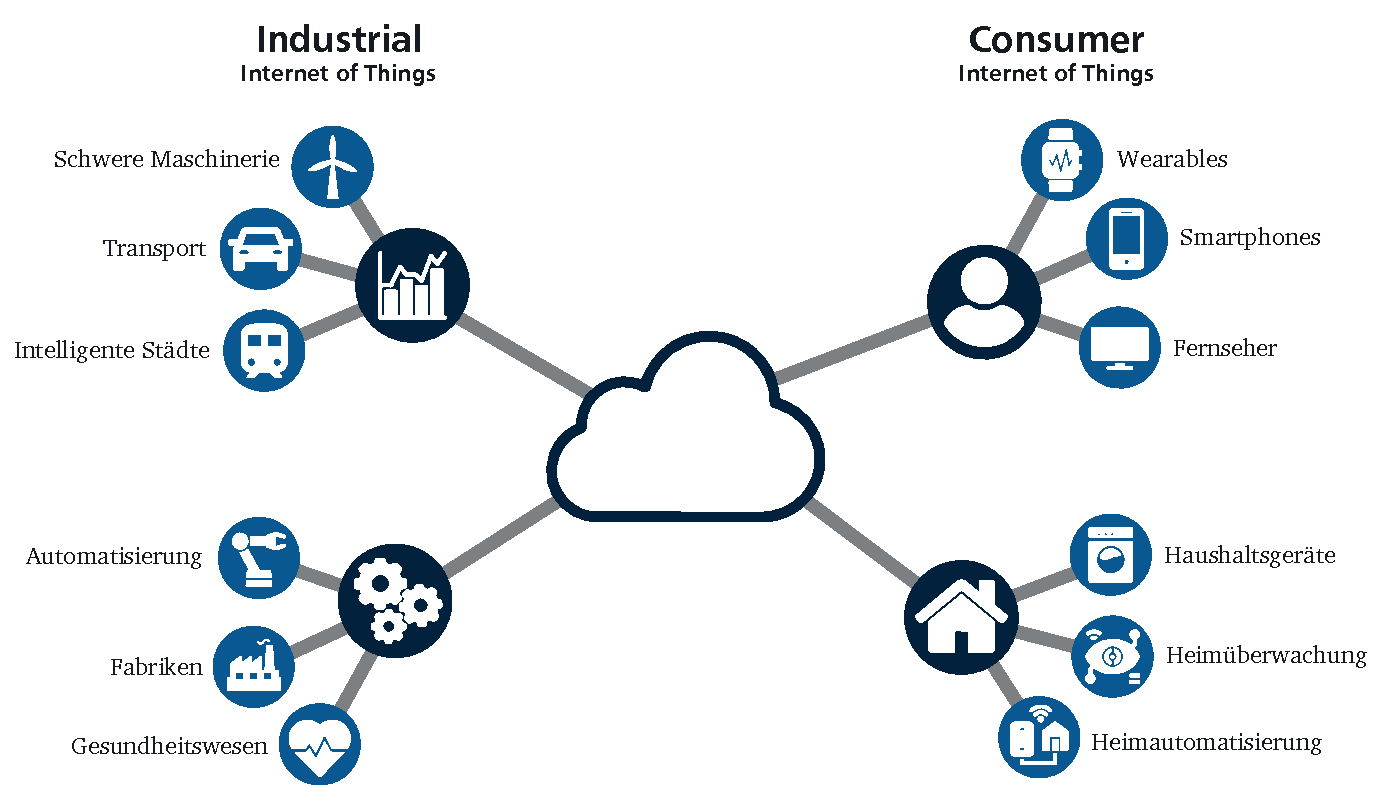
\includegraphics[width=1.0\textwidth]{images/02/IIoT_vs_IoT.pdf}
    \caption{Vergleich zwischen industriellem und Massenmarkt-IoT}
    \label{fig:IIoT_vs_IoT}
\end{figure}

IIoT verfügt über eine Referenzarchitektur vom Industrial Internet Consortium (IIC), welche in die folgenden drei Ebenen unterteilt ist [\cite{iiotReference}]:
\begin{enumerate}
    \item \textbf{Edge} – Die Edge-Schicht liegt direkt an der Anlage. Sie ist dafür verantwortlich, Daten von den Edge-Geräten zu sammeln und sie stromaufwärts zur Platform-Schicht zu übertragen.
    \item \textbf{Platform} – In der Platform-Schicht sind Verwaltungsfunktionen sowie Datenanalyse und -auswertungen angesiedelt.
    \item \textbf{Enterprise} – Die Enterprise-Schicht stellt eine Schnittstelle zum Endbenutzer dar und implementiert verschiedene Entscheidungsunterstützungssysteme und Anwendungen.
\end{enumerate}

Neben dieser Referenzarchitektur wurde von verschiedenen Seiten weitere Architekturen vorgeschlagen, doch in dieser Arbeit wird der Fokus vorwiegend auf einem Aufbau liegen, welcher nah an der Referenzarchitektur liegt. Dies geht unter anderem darauf zurück, dass sich die drei Schichten gut auf die typische Softwarestruktur mit einem Backend, einer Middleware, und einem Frontend übertragen lässt.

Durch die Integration verschiedener Softwarealgorithmen, welche die Systeme autonom optimieren können, verspricht das IIoT-Paradigma, die Betriebseigenschaften technischer Systeme zu verbessern. Zu diesen Eigenschaften zählen unter anderem Kostenreduktionen, Energieverbrauch, Durchsatz und Zeiteffizienz. [\cite{iotApplications}]
 
